\chapter{Experimentelle Aspekte\label{chap:3}}
\begin{compactitem}
\item Messgröße für Vergleich Experiment - Theorie
\item Durchgang von Teilchen durch Materie\\
$\ra$ Teilchennachweis
\item Biologische Strahlenwirkung\\
$\ra$ Dosimetrie
\end{compactitem}
\section{Wirkungsquerschnitt und Lebensdauer}
\tb{Wirkungsquerschnitt (WQ)}\\
= \glqq effektive Trefferfläche\grqq{} für Reaktion zweier Teilchen

\begin{figure}[!ht]
\centering
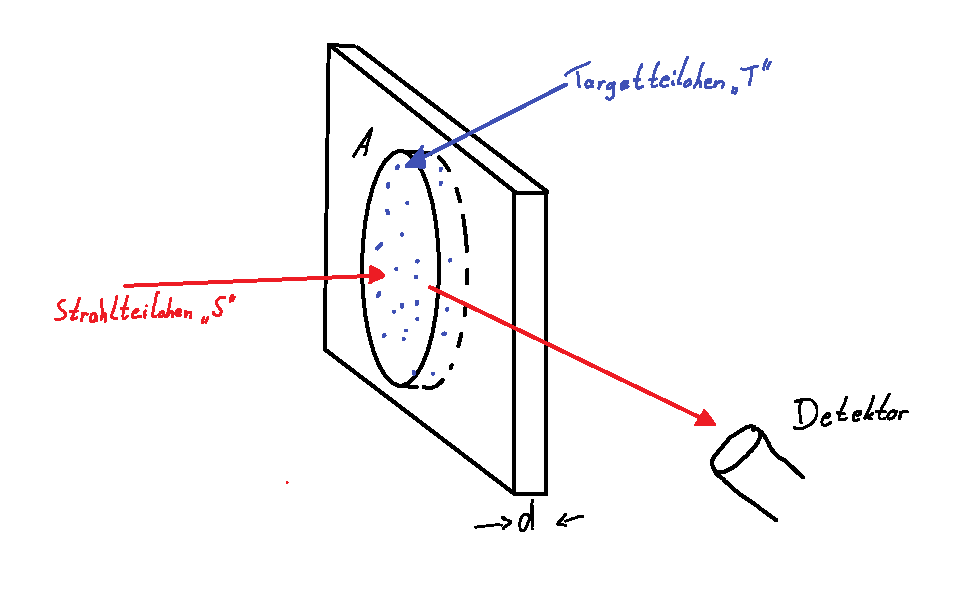
\includegraphics[width=.5\textwidth]{imgs/ep5-fig-3-1.pdf}
\caption{Bestrahlung eines Streuobjektes und anschließender Detektion der gestreuten Teilchen}
\end{figure}
Strahlteilchen streuen an dem Volumen $A\cdot d$ ($A$: Streufläche, $d$: Streudicke). Beschreibe Strahlteilchen durch Stromdichte $j_S= \frac{\Delta N_S}{A\Delta t}$ und Targetteilchen durch Dichte $\rho_T =\frac{N_T}{V}= \frac{N_T}{Ad}$. Die Zahl der Reaktionen ist dann
\begin{align}
\boxed{\frac{\Delta N_{WW}}{\Delta t} = \frac{\Delta N_S}{\Delta t}N_T \cdot \underbrace{\frac{\sigma_{ST}}{A}}}\\
\text{\footnotesize WW-Wskt. pro WW-Versuch} \nonumber
\end{align}
$\Delta N_S \cdot N_T $ = Zahl der WW-Versuche.\\
$\sigma_{ST} = $ WQ für $S$-$T$-WW und hängt von der Art der Teilchen $S$, $T$ sowie von $E_\mr{CMS}$ ab, $\left[\sigma_{ST}\right] = \mr{m^2}$. Mit $\dot{N}_{WW}$ als WW-Rate lässt sich schreiben
\begin{align}
\Ra \boxed{ \sigma_{ST} = \frac{\dot{N}_{WW}}{j_S\cdot N_T} }
\end{align}
\begin{figure}[!ht]
\captionsetup{type=figure}
\centering
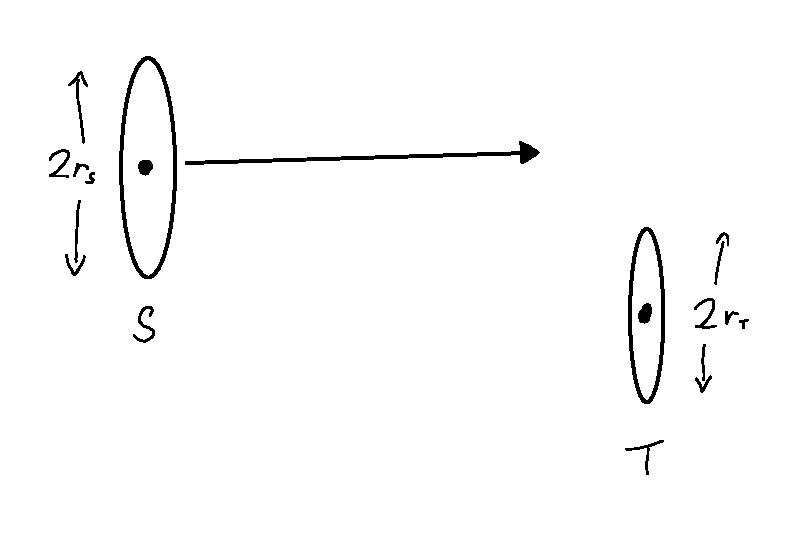
\includegraphics[width=.5\textwidth]{imgs/ep5-fig-3-2.pdf}
\caption{Geometrische Interpretation des WQ}
\end{figure}
Durch eine geometrische Interpretation des WQ (zwei Kugeln stoßen), würde man klassisch erhalten:
\begin{align}
\Ra \sigma_{ST}^{geo}= \pi \left( r_S + r_T\right)^2
\end{align}
Dies gilt jedoch \tb{nur} für ausgedehnte Objekte, aber nicht für Elementarteilchen.
\begin{framed}
\tb{Einheit von $\sigma$}: $1\,\mr{barn}=1\,\mr b = 10^{-28}\,\mr{m^2}$
\end{framed}
\begin{itemize}
\item Beispiel 1: $p+p \ra X$
\begin{align}
\begin{split}
r_p = 10^{-15}\,\mr{m}\\
\Ra \sigma_{pp}^{geo} = 4\pi r_p^2 = 1.2 \cdot 10^{-29}\,\mr{m^2} = 120\,\mr{mb}
\end{split}
\end{align}
Gemessen: $\sigma_{pp}^{exp}$ ist energieabhängig und kleiner
\begin{align*}
\sigma^{tot} = \sigma^{el} + \sigma^{Coul}
\end{align*}
\begin{center}
\captionsetup{type=figure}
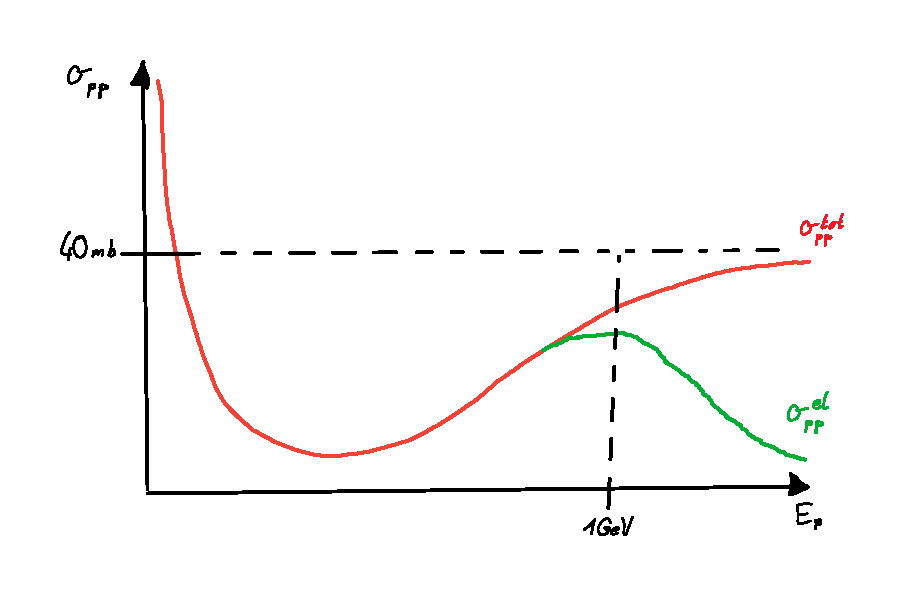
\includegraphics[width=.5\textwidth]{imgs/ep5-fig-3-3.pdf}
\captionof{figure}{Abhängigkeit des WQ von der Energie (hier für $pp$-WW)}
\end{center}

\item Beipiel 2: $\nu+p \ra X$\\
Wenn $r_\nu = 0 \Ra \sigma_{\nu p}^{geo} = 30$\,mb. Gemessen:
\begin{align}
\boxed{\sigma_{\nu p}^{exp} = 0.7\cdot 10^{-42}\,\mr{m^2}}
\end{align}
$\lt$ Faktor $\sim 10^{-13}$!
\item[$\Ra$] WQ in Teilchenphysik ist i.A. \tb{nicht} durch Geometrie der Teilchen gegeben
\item[$\Ra$] WQ ist \tb{stark} energieabhängig
\end{itemize}

 \tb{Differentieller WQ}\\
Effektive Trefferfläche für den Endzustand in einem bestimmten kinematischen Intervall, z.B. Raumwinkel.
\begin{figure}[!ht]
\centering
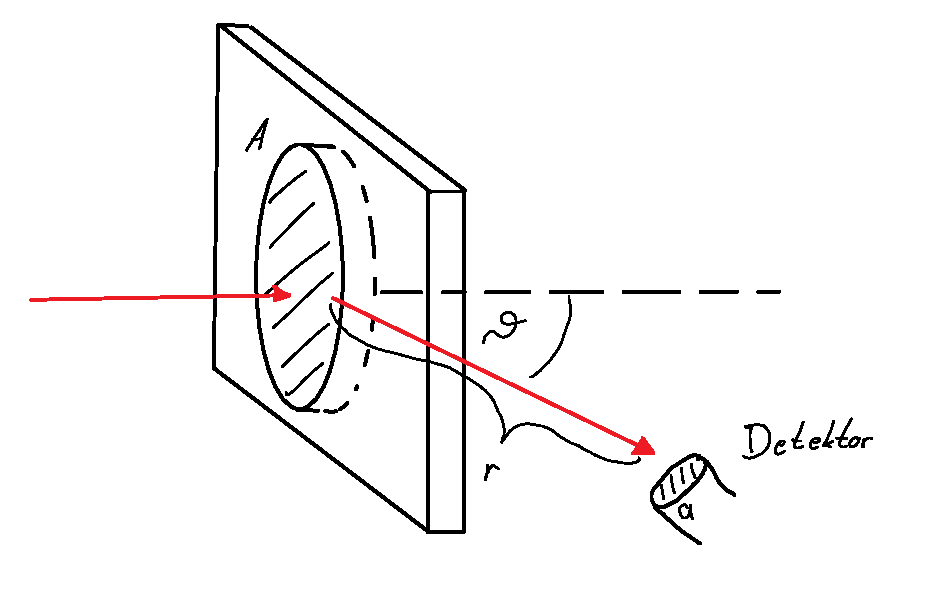
\includegraphics[width=.5\textwidth]{imgs/ep5-fig-3-4.pdf}
\caption{Skizze zur Raumwinkeldetektion}
\end{figure}

  Es gilt hier:
\begin{align}
\begin{split}
\Delta \Omega = \frac{a}{r^2}\\
\Ra \frac{\Delta N_{WW}}{\Delta t} = \frac{N_S}{\Delta t} \cdot N_T \cdot \frac{\Delta \sigma_{ST}^{\Delta \Omega}}{A}\\
\boxed{ \Delta \sigma = \frac{\Pa \sigma_{ST}}{\Pa \Omega}\cdot \Delta \Omega }
\end{split}
\end{align}
Der differentielle WQ ist also:
\begin{align}
\frac{\Pa \sigma_{ST}}{\Pa \Omega} = \underbrace{\frac{\Delta N_{WW}}{\Delta \Omega}}_\text{Messgröße} \cdot \underbrace{\frac{A}{N_S N_T}}_\text{Aufbau}
\end{align}
\begin{framed}
\tb{Anmerkung:}\\
Der WQ ist lorentzinvariant, der differentielle WQ jedoch nicht, da $\Pa \Omega$ variant ist.
\end{framed}

 \tb{Berechneter WQ}
\begin{align}
\begin{split}
\sigma &\sim \labs M \rabs ^2 \rho_Z\\
\delfrac{}{k} \sigma &\sim \labs M \rabs^2 \dfrac{}{k} \rho_Z
\end{split}
\end{align}
\begin{compactitem}
\item $\rho_Z$: Endzustandsdichte (\glqq Zahl der möglichen QM-Wellefunktionen\grqq{})
\item $k$: kinematische Variable
\end{compactitem}
Im Allgemeinen ist die Proportionalität bekannt.

\tb{Lebensdauer}\\
Kerne und Teilchen können instabil sein
\begin{align}
\lambda = \frac{\Pa \left(\text{Zerfallswahrscheinlichkeit}\right)}{\Pa t} = \text{Zerfallskonstante}
\end{align}
\begin{itemize}
\item[$\lt$] $\lambda$ hängt \tb{nicht} von Vorgeschichte ab
\item[$\lt$] Bei $t=0$: $N_0$ zerfallende Kerne/Teilchen
\begin{align}
\begin{split}
\Pa_t N = \dot{N} = -\lambda N\\
\Ra \boxed{ N(t) = N_0 e^{-\lambda t} }
\end{split}
\end{align}
\item[$\lt$] \tb{Mittlere Lebensdauer}
\begin{align}
\boxed{\tau = \frac{\int N(t) \cdot t \,\Pa t}{\int N(t) \, \Pa t} = \frac{1}{\lambda}}
\end{align}
\item[$\lt$] \tb{Halbwertszeit}
\begin{align}
\begin{split}
N\left(T_{\nicefrac{1}{2}}\right) = \frac{1}{2}N_0\\
\Ra T_{\nicefrac{1}{2}} = \frac{\ln 2}{\lambda} = \tau \cdot \ln 2
\end{split}
\end{align}
\item[$\lt$] mehrere Zerfallskanäle $i = 1, \dots, n$; $\lambda_1,\dots,\lambda_n$
\begin{align}
\begin{split}
\Lambda = \sum_i^n \lambda_i\\
N(t) = N_0 e^{-\Lambda t}\\
\tau = \Lambda^{-1} = \frac{1}{\sum_i^n \lambda_i}\\
BR_i = \frac{\lambda_i}{\Lambda}
\end{split}
\end{align}
$BR_i$: Branching-Ratio\\
Berechnung:
\begin{align}
\lambda \sim \labs M\rabs^2 \rho_Z
\end{align}
Auch hier ist die Proportionalität bekannt.
\end{itemize}
\section{Wechselwirkung von Teilchen mit Materie}
\begin{itemize}
\item[$\lt$] Prozesse, die messbare Signale erzeugen
\item[$\lt$] Hier: elm. Prozesse = WW von Photonen oder geladenen Teilchen mit Elektronen oder elm. Kern-Feldern betrachten wir im Weiteren $e^-$ als ungebunden oder (quasi) frei
\end{itemize}
Photonen:
\begin{compactitem}
\item Photoionisation
\item Compton-Streuung
\item Paarbildung
\end{compactitem}
geladenen Teilchen:
\begin{compactitem}
\item Ionisation
\item Bremsstrahlung
\item Cherenkowstrahlung
\end{compactitem}
Anwendungen in Teilchendetektion, Medizin oder auch Materialwissenschaften.

\tb{Photoionisation} (vgl. \autoref{fig:3.5})\\
Photon $\gamma$ wird absorbiert und überträgt $E_\gamma$ auf $e^-$.
\begin{align*}
\boxed{ \gamma + \text{Atom} \ra e^- + \left(\text{Atom}\right)^+ }
\end{align*}
Der Effekt ist dominant für $E_\gamma \lesssim 30$\.keV (Röntgen)
\begin{align*}
\sigma_{p_i} \sim Z^5 E_\gamma^{-3.5}
\end{align*}
\begin{itemize}
\item[$\lt$] Zunahme $\sigma_{p_i}$, wenn tiefer liegende Schalen \glqq zugänglich\grqq{} werden (Absorptionskanten)
\item[$\lt$] schwere Elemente schirmen \tb{viel} besser ab ($\ra$ Pb)
\end{itemize}
\begin{minipage}[c]{.45\textwidth}
\captionsetup{type=figure}
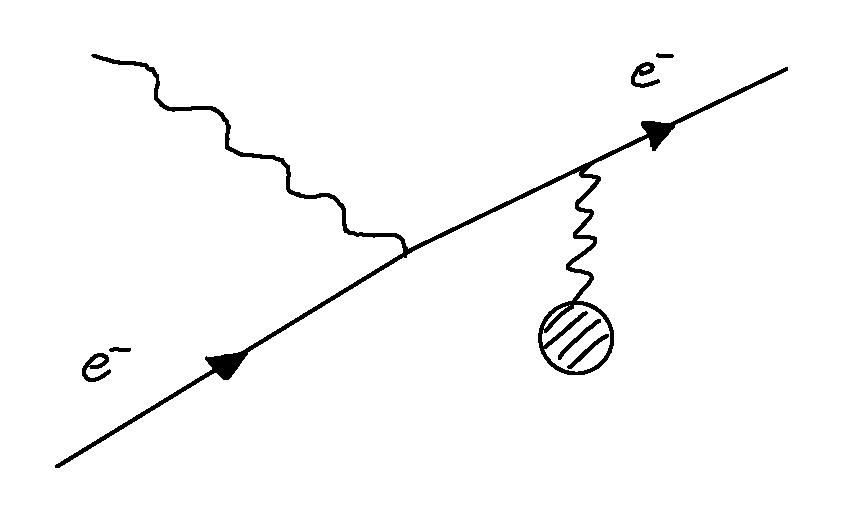
\includegraphics[width=\textwidth]{imgs/ep5-fig-3-5.pdf}
\captionof{figure}{Feynmandiagramm der Photoionisation\label{fig:3.5}}
\end{minipage}
\begin{minipage}[c]{.45\textwidth}
\captionsetup{type=figure}
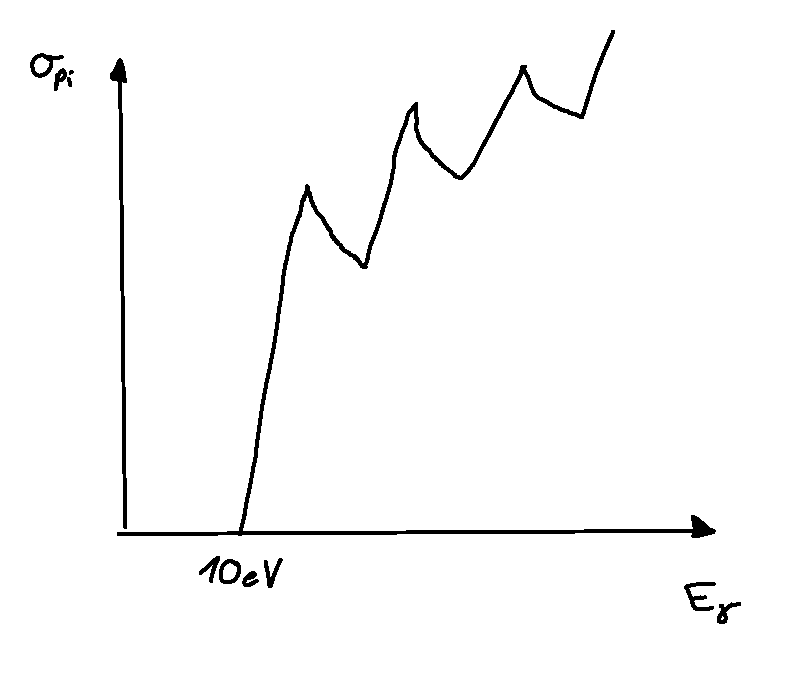
\includegraphics[width=\textwidth]{imgs/ep5-fig-3-6.pdf}
\captionof{figure}{Schematisches Absorptions-\\spektrum}
\end{minipage}

\tb{Compton-Streuung} (vgl. Abb.\ref{fig:3.7})\\
elastische Streuung, Energieübertrag auf $e^-$
\begin{align*}
\boxed{ \gamma + e^- \ra \gamma + e^- }
\end{align*}
Dominant für 30\,keV$\leq E_\gamma \leq$ 5\,MeV\\
$\Ra$ Wellenlänge ändert sich durch $\gamma$
\begin{align*}
\boxed{ \Delta \lambda = \frac{h}{m_e c} \left( 1 - \cos \theta \right) \ \ \ \forall E_\gamma }\\
\lambda_C= \frac{h}{m_e c} \approx 2.4\cdot 10^{-12}\,\mr{m}
\end{align*}
$\lambda_C$ Compton-Wellenlänge des Elektrons\\
Für $\nicefrac{E_\gamma}{m_e} \gg 1$:
\begin{align*}
\sigma_C \sim \alpha^2 \frac{1}{E_\gamma}\ln \left( \frac{2 E_\gamma}{m_e}\right)
\end{align*}

\begin{figure}[!ht]
\centering
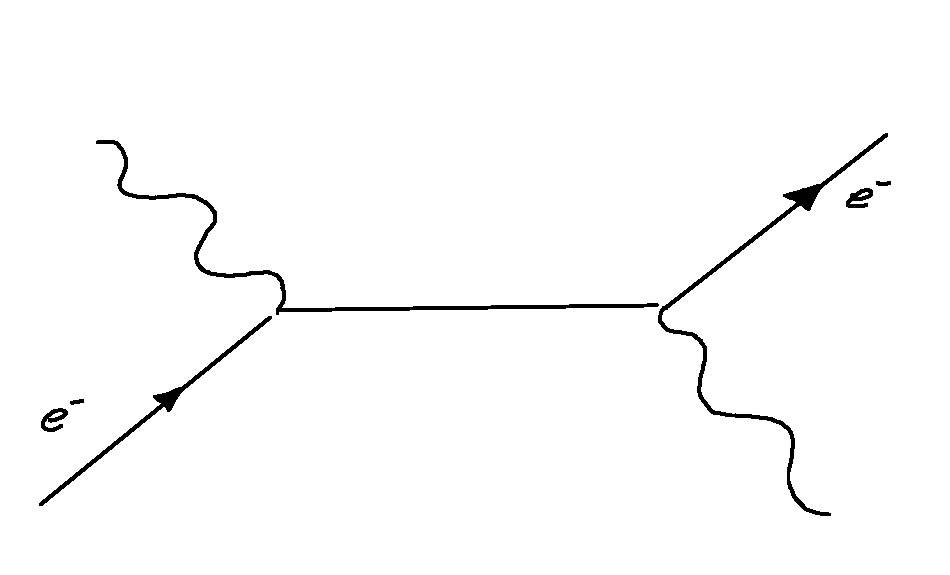
\includegraphics[width=.5\textwidth]{imgs/ep5-fig-3-7.pdf}
\caption{Feynmandiagramm der Compton-Streuung\label{fig:3.7}}
\end{figure}

 \tb{Paarbildung} (vgl. Abb.\ref{fig:3.8})
\begin{align*}
\boxed{ \gamma + \text{Kern} \ra e^+e^-+\text{Kern} }
\end{align*}
  Energieschwelle $E_\gamma > 2m_e \approx 1$\,MeV
\begin{align*}
\sigma_p \sim Z^2 \ln \frac{E_\gamma}{m_e}
\end{align*}
$\Ra$ dominant bei (sehr) hohen Energien

\begin{minipage}[c]{.45\textwidth}
\captionsetup{type=figure}
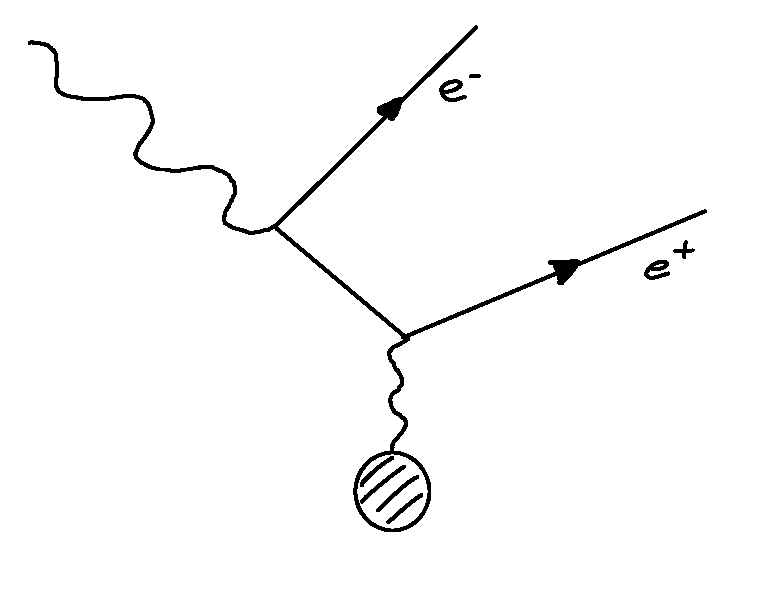
\includegraphics[width=\textwidth]{imgs/ep5-fig-3-8.pdf}
\captionof{figure}{Feynmandiagramm der\\ Paarbildung\label{fig:3.8}}
\end{minipage}
\begin{minipage}[c]{.45\textwidth}
\captionsetup{type=figure}
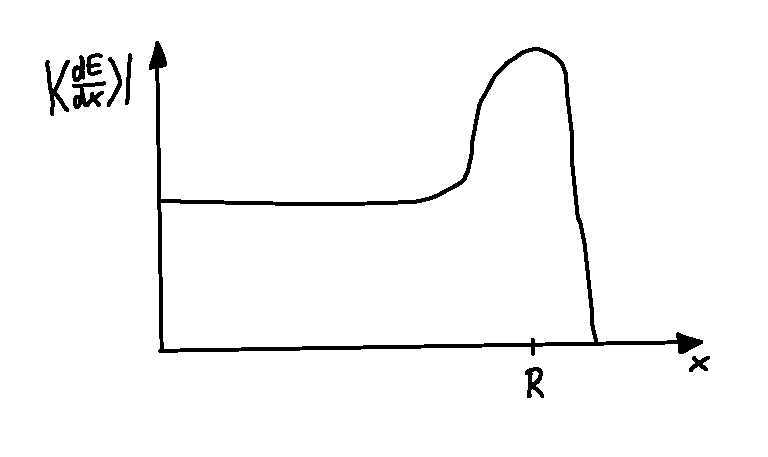
\includegraphics[width=\textwidth]{imgs/ep5-fig-3-9.pdf}
\captionof{figure}{Bragg-Peak visualisiert als\newline  Energieverlust für eine bestimmte Eindringtiefe\label{fig:3.9}}
\end{minipage}

\tb{Ionisation} (vgl. Abb. \ref{fig:3.9})

Am Ende des Abbremsvorgangs hoher Energieverlust $\sim \frac{1}{\beta^2}$ $\Rightarrow$ \glqq Bragg-Peak\grqq{}

\tb{Bremsstrahlung}
	\begin{align}
	\boxed{T+ \text{Kern}\rightarrow T+ \text{Kern}+\gamma}
	\end{align}
Energieverlust:
	\begin{align}
	\boxed{-\left\langle \dfrac{E}{x}\right\rangle_{\text{Brems}}=\frac{E}{x_0}}
	\end{align}
$x_0$: Strahlungslänge (materialabhängig)
	\begin{align}
	\boxed{\frac{1}{x_0}\sim \underbrace{nZ^2}_{\text{Material}} \cdot \frac{Z^2_s}{M^2}}
	\end{align}
$x_0=36\,cm$ für $e^-$ in $H_2O$ und $x_0=5,6\,mm$ für $e^-$ in $Pb$
\begin{itemize}
\item[$\ra$] $E(x)=E(x=0)\cdot e^{-\frac{x}{x_0}}$ ausschließlich Bremsstrahlung
\item[$\ra$] besonders stark für $e^-$ (kleine Masse)
\item[$\ra$] $x_0$ auch für Paarerzeugung: Mithilfe freier Weglänge $=\frac{7}{9}x_0$
\end{itemize}

	\begin{figure}[!ht]
	\centering
	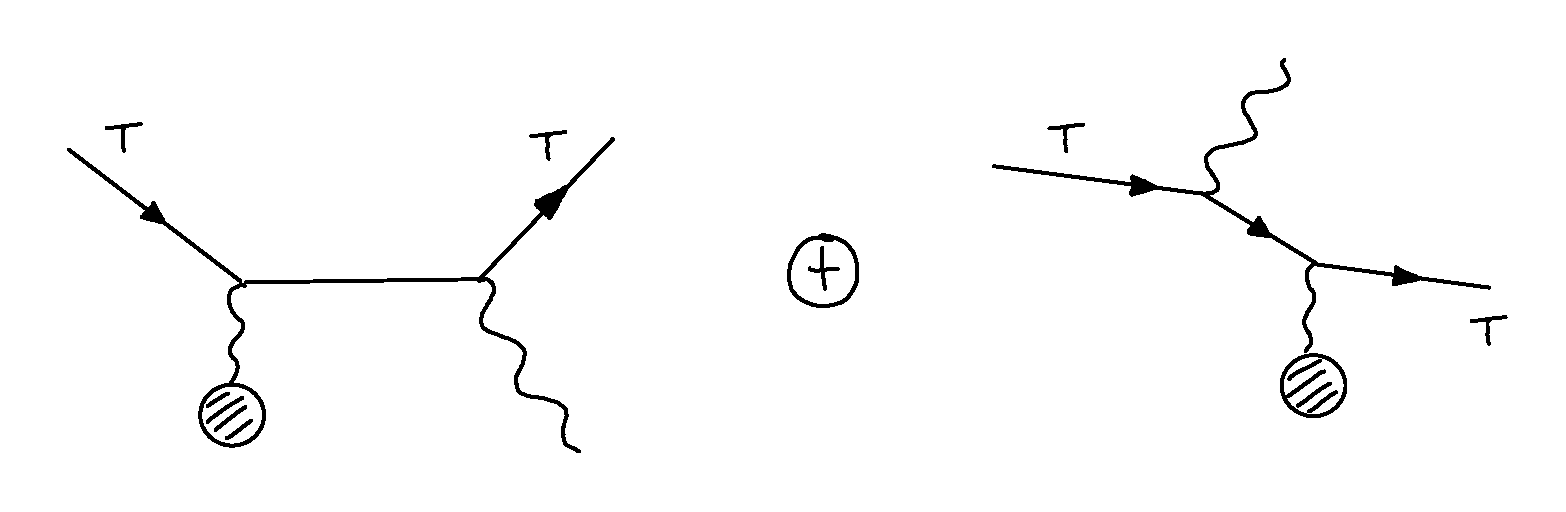
\includegraphics[width=.6\textwidth]{imgs/ep5-fig-3-10.pdf}
	\caption{Feynmandiagramme der Bremsstrahlung (für $T=e^-$, \glqq topologisch äquivalent zu Paarerzeugung\grqq ) \label{fig:3.10}}
	\end{figure}

\tb{Cherenkov-Strahlung}
	\begin{align}
	v_{\text{Teilch}}>v_{\text{Phase}}
	\end{align}
Durchgang geladener Teilchen durch transparente Medien (Brechungsindex n) mit $\beta >\frac{1}{n}$\\
Lichtemission. Aus Abb. \ref{fig:3.11} folgt geometrisch der Zusammenhang
\begin{align}
\boxed{cos\theta_c=\frac{1}{\beta n}}
\end{align}
\begin{itemize}
\item[$\ra$] Winkel für den Teilchennachweis verwendet
\item[$\ra$] Beitrag $2u\frac{dE}{dx}$ ist sehr klein
\end{itemize}
	\begin{figure}[!ht]
	\centering
	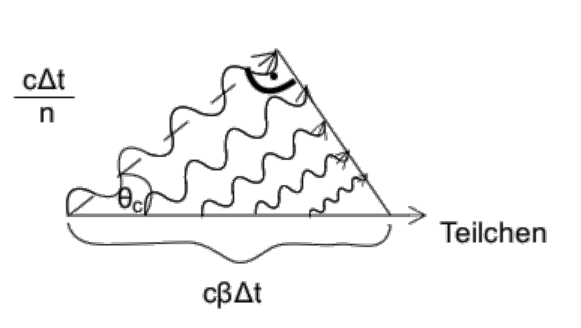
\includegraphics[width=.5\textwidth]{imgs/ep5-fig-3-11.pdf}
	\caption{Cherenkov-Strahlung mit charakteristischem Cherenkovkegel \label{fig:3.11}}
	\end{figure}

\textbf{Absorption von Photonen}
\begin{align}
\begin{split}
\Pa N =-W_a\cdot N =-\frac{\sigma \cdot N_T}{A}\cdot N=-\frac{\sigma n_T A\Pa x}{A}\cdot N\\
\Rightarrow \frac{dN}{dx}=-\underbrace{\sigma n_T}_{= \mu} N\\
\Rightarrow \boxed{N(x)=N_0 e^{-\mu x}}
\end{split}
\end{align}
\begin{compactitem}
\item[mit] $W_a$: Absorptionswahrscheinlichkeit
\item[] $\mu$ Absorptionskoeffizient
\end{compactitem}
\begin{itemize}
\item[$\ra$] Mittlere freie Weglänge
\begin{align}
\boxed{\lambda=\frac{1}{\mu}=\frac{1}{\sigma n_T}}
\end{align}
\item[$\ra$] Häufig angegeben:
\begin{align}
\boxed{\mu'=\frac{\mu}{\rho}=\frac{n_T}{\rho}\cdot \sigma=\frac{N_A}{M_m}\sigma}
\end{align}
\end{itemize}
	\begin{figure}[!ht]
	\centering
	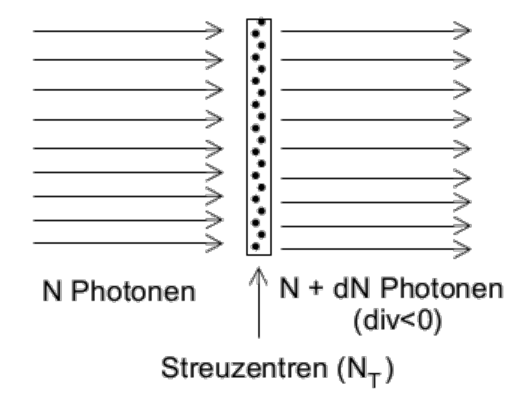
\includegraphics[width=.45\textwidth]{imgs/ep5-fig-3-12.pdf}
	\caption{Absorption von Photonen beim Durchgang durch ein Medium\label{fig:3.12}}
	\end{figure}

\section{Grundbegriffe der Dosimetrie}
Hier lediglich einige Grundbegriffe, \textbf{keine} Messverfahren.
Einfluss von Strahlenbelastung auf biologische Organismen
\begin{itemize}
\item[$\ra$] \textbf{Aktivität}
\begin{align}
\boxed{A=\left\langle\left|\frac{dN}{dt}\right|\right\rangle=
\frac{\text{mittlere Zahl von Zerfällen}}{\mr s}}
\end{align}
\begin{itemize}
\item[$\ra$] charakterisiert Stärke einer Strahlungsquelle
\item[$\ra$] $[A]=\nicefrac{1}{\mr{s}}=\mr{Bq}=$Becquerel
\item[$\ra$] Bsp.: $^{40}K$-Zerfall im menschlichen Körper $A\sim 10^4\,Bq$ (ca. $10\,\%$ der nat. Strahlenbelastung)\\
\end{itemize}
\item[$\ra$] \textbf{Strahlungsleistung} $A\cdot E$, mit $E$ als freigesetzter Energie pro Zerfall
\item[$\ra$] \textbf{Energiedosis}\\
In Absorber deponierte Energie/Masse
\begin{align}
\boxed{D=\frac{dE}{dM}=\frac{1}{\rho}\frac{\Pa E}{\Pa V},[D]=\mr{\frac{J}{kg}}=\mr{Gy}=\text{Gray}}
\end{align}
(alt: $1\,\mr{Gy}=100\,\mr{rad}$)
\begin{itemize}
\item[$\ra$] Produktion von Sekundärteilchen, chemische Radikale
\item[$\ra$] Schädigung der DNA $\rightarrow$ Mutationen
\item[$\ra$] $\alpha-,\beta-,\gamma-$Strahlung ($\rightarrow$ Kap 5) wirken sehr unterschiedlich schädigend
\end{itemize}
\item[$\ra$]\textbf{Äquivalentdosis}
\begin{align}
\begin{split}
H=D\cdot Q\\
[H]=\mr{\frac{J}{kg}}=\mr{Sv}=\text{Sievert}\\
Q=\begin{cases}
1 & \text{für } e^\pm,\gamma\\
10 & \text{für schnelle }n \\
20 & \text{für }\alpha-\text{Teilchen, Kerne}
\end{cases}
\end{split}
\end{align}
$Q$ = relative, biologische Wirksamkeit=\glqq Qualitätsfaktor\grqq\\
(alt: $1\,\mr{Sv}=100\,\mr{rem}$)
\item[$\ra$] \textbf{Typische Dosen}\\
Natürliche Strahlenbelastung (Gestein): $1\,\mr{\frac{mSv}{a}}$\\
Transatlantikflug: $50-100\,\mu \mr{Sv}$\\
Computertomographie: $10\,\mr{mSv}$\\
Höchstgrenze Strahlenschutzverordnung $20\,\mr{\frac{mSv}{a}}$\\
Letale Dosis: $6\,\mr{Sv}$

Achtung: Gesundheitswirkung:
\begin{itemize}
\item[$\ra$] hängt davon ab, in welchem Organ Strahlung deponiert wird
\item[$\ra$] ist besonders stark bei inkorporierten Quellen
\end{itemize}
\end{itemize}